\newcommand{\env}[1]{\texttt{#1}}
\newcommand{\command}[1]{\texttt{#1}}
\newcommand{\package}[1]{\texttt{\itshape#1}}
\newcommand{\engl}[1]{(engl: \textit{#1})\xspace}
\setlength{\parindent}{0pt}
\lstset{extendedchars=\true}
\lstset{inputencoding=ansinew}
\newpage

\section{Aufgabe 2}\cite{[1]}

\subsection{Frage- bzw. Aufgabenstellung}

Unter Verwendung der in der Einleitung erwähnten Daten sollen Sie in Java einen Clienten erstellen, der für einen beliebigen Ort die maximale- (tx) und minimale Temperatur (tn) anzeigen kann. Die restlichen Informationen müssen nicht berücksichtigt werden.

\subsection{Lösung}

Für die Lösung dieser Aufgabe wurde eine Klasse mit dem Namen \textit{MaxMinTemp} erstellt in der alle Methoden, inklusive der main-Methode, realisiert wurden. \\
\\
Zunächst wurde eine \textit{readUrl}-Methode geschrieben, der man eine URL-Adresse übergibt und alle Zeichen auf dieser Seite einem StringBuilder hinzufügt und diesen dann auch zurückgibt (siehe Zeile 1 bis 16).

\begin{lstlisting}[caption={readUrl-Methode}]
private static String readUrl(String urlString) throws Exception {

	BufferedReader reader = null;
	try {
		URL url = new URL(urlString);
		reader = new BufferedReader(new InputStreamReader(url.openStream()));
		StringBuilder sb = new StringBuilder();
		int read;
		while ((read = reader.read()) != -1)
			sb.append((char) read);
		return sb.toString();
	} finally {
		if (reader != null)
			reader.close();
	}
}
\end{lstlisting}

Weiterhin wurde eine \textit{getDate}-Methode geschrieben, die später dazu benötigt wird, um später nur die Temperaturen für den aktuellen Tag anzuzeigen. Hierfür wird das richtige Format mit einem Objekt von \textit{DateFormat} gesetzt. Danach wird ein neues Datum erzeugt und mit dem richtigen Format zurückgegeben (siehe Zeile 1 bis 5).

\begin{lstlisting}[caption={getDate-Methode}]
private static String getDate() {
	DateFormat dateFormat = new SimpleDateFormat("yyyy-MM-dd");
	Date date = new Date();
	return dateFormat.format(date);
}
\end{lstlisting}

Die letzte Methode namens \textit{ausgabeTemp} übernimmt den wichtigsten Teil der Aufgabe, da sie dafür sorgt, dass wir am Ende die Ausgaben der Temperaturen auf der Konsole haben. Da wir hier mit dem JSON-Format arbeiten, benutzen wir das \textit{org.json}-package, um mit den JSON-Objekten zu arbeiten.\cite{[2]} \\
\\
Zu Beginn wird der \textit{Scanner} benutzt, damit der Benutzer den Namen, so wie die Postleitzahl der Stadt eingeben kann, für die der Benutzer die Wetterausgabe haben will. Anschließend wird ein neues JSONObject erstellt, dem man dann mithilfe der \textit{readUrl}-Methode die API der OpenWeatherMap zusammen mit der zuvor eingegebenen Stadt (plus zugehöriger Postleitzahl) übergibt (siehe Zeile 1 bis 9). \\
\\
Da die Daten im JSON-Format immer in einer untergeordneten Sammlung über Name/Werte-Paare gespeichert sind, muss man zunächst gucken wie man an die Temperaturen der API kommt. Dazu eignet sich die Seite \url{https://jsonformatter.curiousconcept.com/} (Vorschlag aus dem Praktikumsblatt. Hier werden die JSON-Daten vernünftig formatiert, so dass man einen guten Überblick über alle Daten bekommt. Wie man in Abbildung 1 sieht, sind die Daten für die Temperatur in einem \textit{main}-Objekt, welches wiederum in einem \textit{list}-Array gespeichert ist. 

\begin{figure}[htbp]
\begin{center}
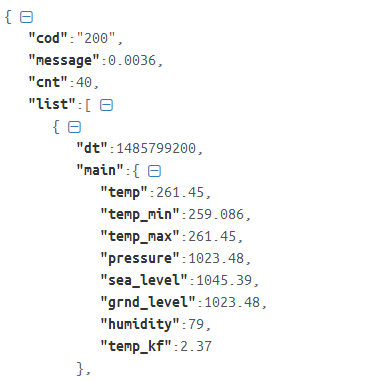
\includegraphics[width=0.7\textwidth]{Bild1}
\caption{Formatierte JSON-Datei der API}
\end{center}
\end{figure}

Mit dem Code aus Zeile 10 bis 13 greifen wir also auf das \textit{main}-Objekt zu und der String \textit{dt\_txt} speichert das Datum der Wettervorhersage. Anschließend erstellt man noch ein String für das aktuelle Datum mit der \textit{getDate}-Methode und das Datum aus dem \textit{dt\_txt} String, welcher jedoch nicht die Uhrzeit enthält (siehe Zeile 14,15). Diese Strings sind später für die Bedingung in der while-Schleife wichtig. Vor der while-Schleife sucht man sich aus der JSON-Datei noch den Namen der Stadt raus, da wir diese mit ausgeben wollen (siehe Zeile 16 bis 18).\cite{[3]} \\
\\
Nun gehen wir in die while-Schleife. Diese wird nur ausgeführt wenn \textit{dateOfForecast} mit \textit{date} übereinstimmt. Dies ist wichtig, da wir die API für die 5-Tage Vorhersage benutzen, aber lediglich die Vorhersage für den aktuellen Tag wollen (siehe Zeile 19). Zeile 20 bis 23 stimmen mit den Zeilen 12 bis 15 überein, daher werden diese nicht nochmal erklärt. Um nun die minimale/maximale Temperatur zu bekommen, müssen wir wie man in Abbildung 1 sieht auf das \textit{main}-Objekt zugreifen und von dort dann auf die Integer-Werte \textit{temp\_min} und  \textit{temp\_max} (siehe Zeile 24 bis 26). Anschließend werden noch alle mit einer üblichen \textit{println} ausgegeben und \textit{i} wird erhöht um auf das nächste \textit{main}-Objekt zuzugreifen (siehe Zeile 27,28).


\begin{lstlisting}[caption={ausgabeTemp}]
private static void ausgabeTemp() throws Exception {
	Scanner scan = new Scanner(System.in);
	System.out.println("Für welche Stadt wollen Sie das Wetter anzeigen?");
	String city = scan.nextLine();
	System.out.println("Geben Sie bitte die Postleitzahl ein: ");
	String zipCode = scan.nextLine();
	scan.close();
	try {
		JSONObject json = new JSONObject(readUrl("http://api.openweathermap.org/data/2.5/forecastq=" + city+ "&zip=" + zipCode + "&units=metric&APPID=722920868a0a0266c859a174da690bc1"));
		JSONArray list = json.getJSONArray("list");
		int i = 0;
		JSONObject main = list.getJSONObject(i);
		String dt_txt = main.getString("dt_txt");
		String date = getDate();
		String dateOfForecast = dt_txt.substring(0, 10);
		JSONObject cityNameObject = json.getJSONObject("city");
		String cityName = cityNameObject.getString("name");
		System.out.println(cityName + " :\n");
		while (dateOfForecast.equals(date)) {
			main = list.getJSONObject(i);
			dt_txt = main.getString("dt_txt");
			date = getDate();
			dateOfForecast = dt_txt.substring(0, 10);
			JSONObject temp = main.getJSONObject("main");
			double tn = temp.getDouble("temp_min");
			double tx = temp.getDouble("temp_max");
			System.out.println("min Temp: " + tn + " C , " + "max Temp: " + tx + " C , " + dt_txt);
			i++;
		}

		} catch (JSONException e) {
			e.printStackTrace();
		}
	}
\end{lstlisting}

In der main-Methode wird dann nur noch die \textit{ausgabeTemp}-Methode aufgerufen.

\begin{lstlisting}[caption={main}]
public static void main(String[] args) throws Exception {
		ausgabeTemp();
}
\end{lstlisting}

Die Ausgabe könnten dann so aussehen: 

\begin{figure}[htbp]
\begin{center}
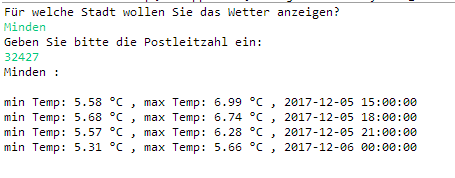
\includegraphics[width=0.7\textwidth]{Bild2}
\caption{Minden, min/max Temperatur}
\end{center}
\end{figure}

\subsection{Ergebnis}

Wir können mithilfe der OpenWeatherMap die Daten für die maximale/minimale Temperatur eines beliebigen Ortes anzeigen.

\section{Quellen}
\begin{thebibliography}{999}
\bibitem {1} OpenWeatherMap, 5 day weather forecast \\ \url{https://openweathermap.org/forecast5}, 4.12.2017

\bibitem {2} org.json, JSON In Java \\ \url{https://mvnrepository.com/artifact/org.json/json}, 4.12.2017

\bibitem {3} vikingmaster, Java - How to get object value in JSON array? \\ \url{https://stackoverflow.com/questions/22386344/java-how-to-get-object-value-in-json-array}, 4.12.2017
\end{thebibliography}







